\chapter{Metodologia}
\label{Metodologia}

Neste capítulo são apresentadas diversas metodologias relacionadas às métricas de busca por inovação, expondo seus parâmetros de busca e fazendo uma breve análise em relação ao potencial de suas aplicações no problema proposto.

\section{Novelty Search}

Algoritmos evolutivos são algoritmos de otimização que convergem soluções em direção à uma função de avaliação global. Em contraste, a Busca Inovativa (\emph{Novelty Search} - NS) \cite{lehman2008exploiting}  \cite{lehman2011abandoning} é uma técnica de evolução divergente baseada na característica de diversificação da evolução natural, a qual é capaz de criar e manter várias espécies que dão suporte à vida. Desta forma a NS recompensa comportamentos inovadores ao invés do progresso em direção à um objetivo fixo, explorando eficientemente o espaço de busca e eventualmente encontrando indivíduos que solucionem o problema, mesmo sem promover um gradiente rumo à nota de avaliação. De fato, a NS vem sendo aplicada de forma eficiente e bem sucedida em diversos problemas \cite{lehman2011evolving} \cite{liapis2013sentient} \cite{woolley2014novel}.

A implementação da NS requer quase nenhuma modificação em qualquer algoritmo evolutivo exceto pela troca da função de avaliação objetiva por uma métrica de inovação, esta tem por sua vez a função de medir o quão diferente um indivíduo é em relação a outros. A ideia principal é que ao invés de recompensar performances em direção a um objetivo, a NS recompensa a diversidade em relação a comportamentos anteriores. As Figuras \ref{fig:ns_diag_ag} e \ref{fig:ns_diag_ns} apresentam as modificações básicas necessárias para a implementação da NS.

\begin{figure}[htb]
	\begin{center}
		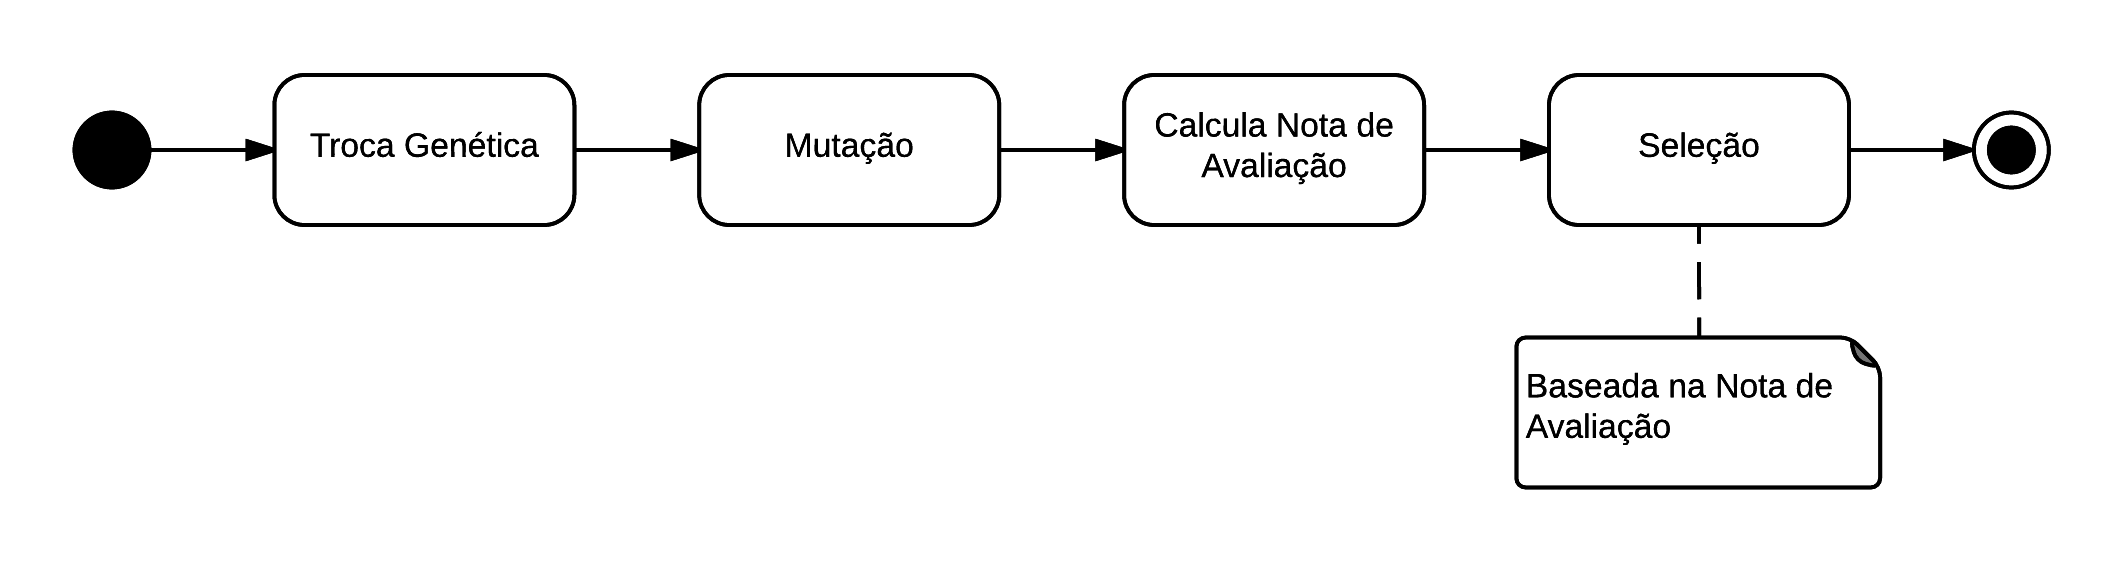
\includegraphics[width=1.0\textwidth]{Imagens/ns_diag_ag.png}
		\caption{Diagrama de Atividades de um típico Algoritmo Genético.}
		\label{fig:ns_diag_ag}
	\end{center}
\end{figure}
 
\begin{figure}[htb]
	\begin{center}
		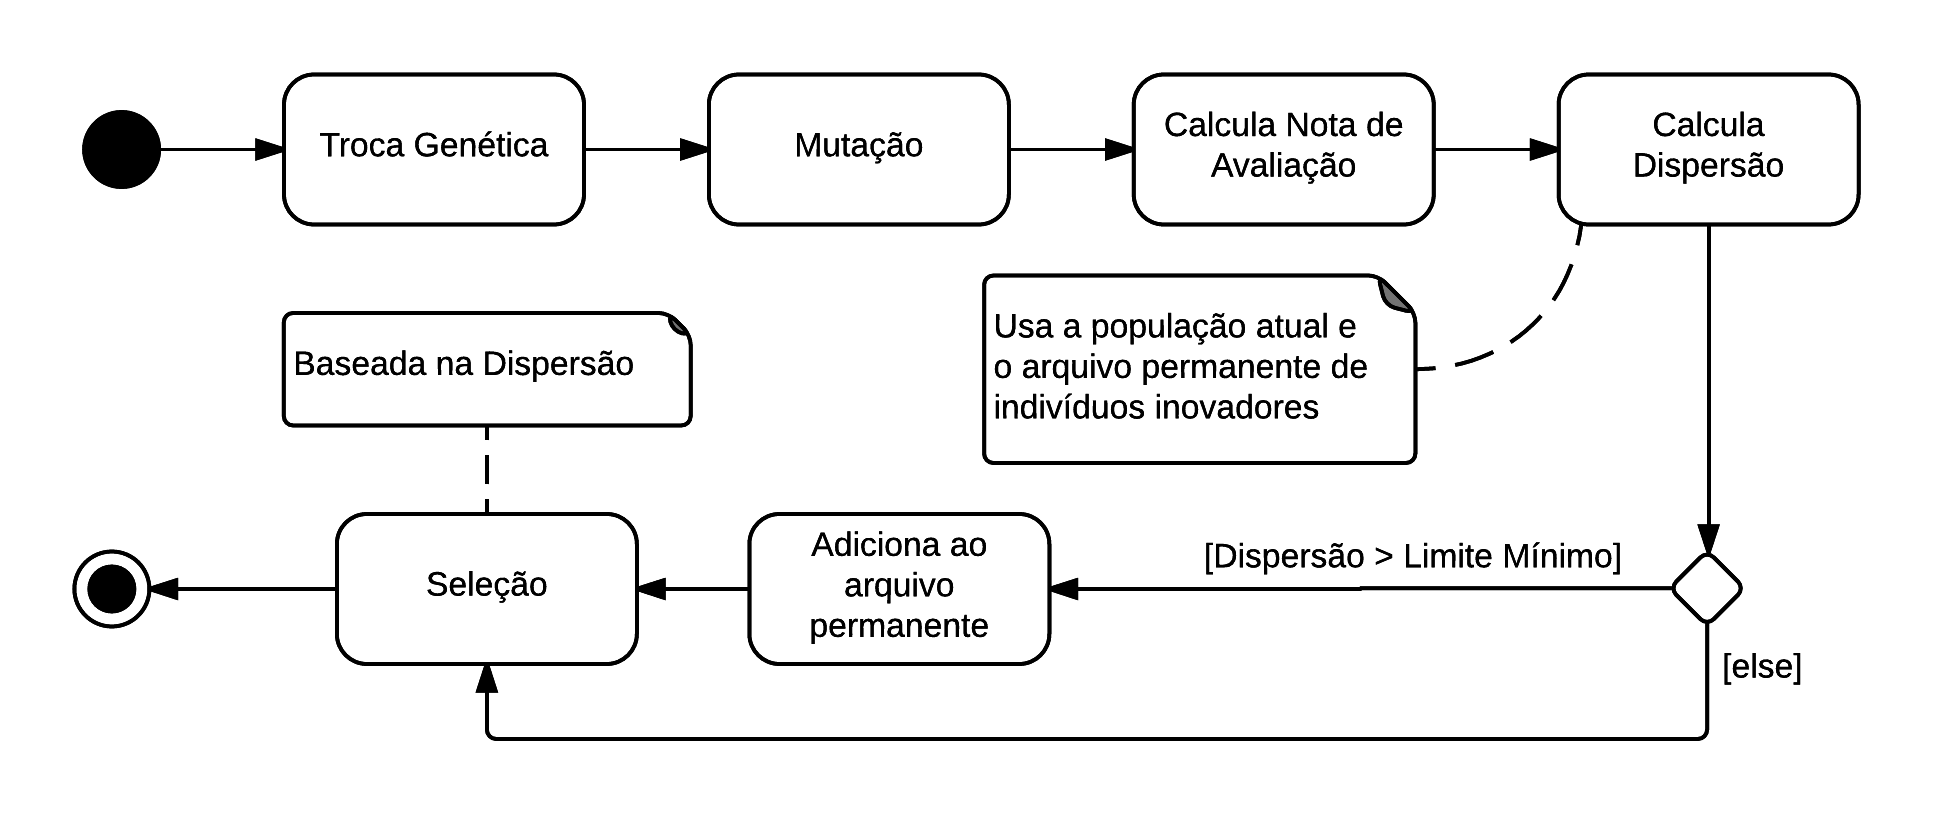
\includegraphics[width=1.0\textwidth]{Imagens/ns_diag_ns.png}
		\caption{Diagrama de Atividades de um Algoritmo Genético de Busca Inovativa.}
		\label{fig:ns_diag_ns}
	\end{center}
\end{figure}

A inovação de um indivíduo recentemente gerado é computada em relação a comportamentos de um arquivo de indivíduos previamente inovadores e à população atual. O arquivo, inicialmente vazio, recebe novos indivíduos quando estes são significativamente diferentes de indivíduos anteriores, i.e., se possuem um valor de inovação acima de um limite computado dinamicamente ou pré-definido.

A métrica de inovação caracteriza o quão distante um indivíduo está em relação ao resto da população atual e seus predecessores no espaço comportamental, baseando-se na dispersão de qualquer ponto neste espaço comportamental. Áreas com altos índices de aglomeração de pontos visitados são menos inovadoras, e portanto menos recompensadas.

Um simples cálculo de dispersão em um certo ponto é a média das distâncias entre este ponto e os $k$-vizinhos mais próximos à ele, onde $k$ é uma constante fixa definida empiricamente. Intuitivamente, se a distância média até os vizinhos mais próximos de um ponto for grande, esta é uma área esparsa; caso seja um valor pequeno, o mesmo está localizado em uma área densa; a Figura \ref{fig:ns_dispersao} representa os pontos P1 e P2 em regiões mais e menos densas respectivamente. A dispersão $\rho$ em um ponto $x$ é dada pela equação \ref{eq:ns_dispersao}
\begin{equation}
    \rho(x) = \frac{1}{k}\sum_{i=0}^kdist(x, \mu_i),
    \label{eq:ns_dispersao}
\end{equation}

\noindent onde $\mu_i$ é o $i$-ésimo vizinho mais próximo de $x$ com respeito a métrica de distância $dist$, que é uma medida de diferença comportamental dependente de domínio entre dois indivíduos no espaço de busca. O cálculo de vizinhos mais próximos deve levar em consideração tanto indivíduos da população atual como do arquivo de indivíduos previamente inovadores. Candidatos em regiões mais esparsas dentro deste espaço de busca comportamental recebem assim maiores valores de inovação, guiando, desta forma, a busca em direção ao que é novo, sem objetivos explícitos.

\begin{figure}[htb]
	\begin{center}
		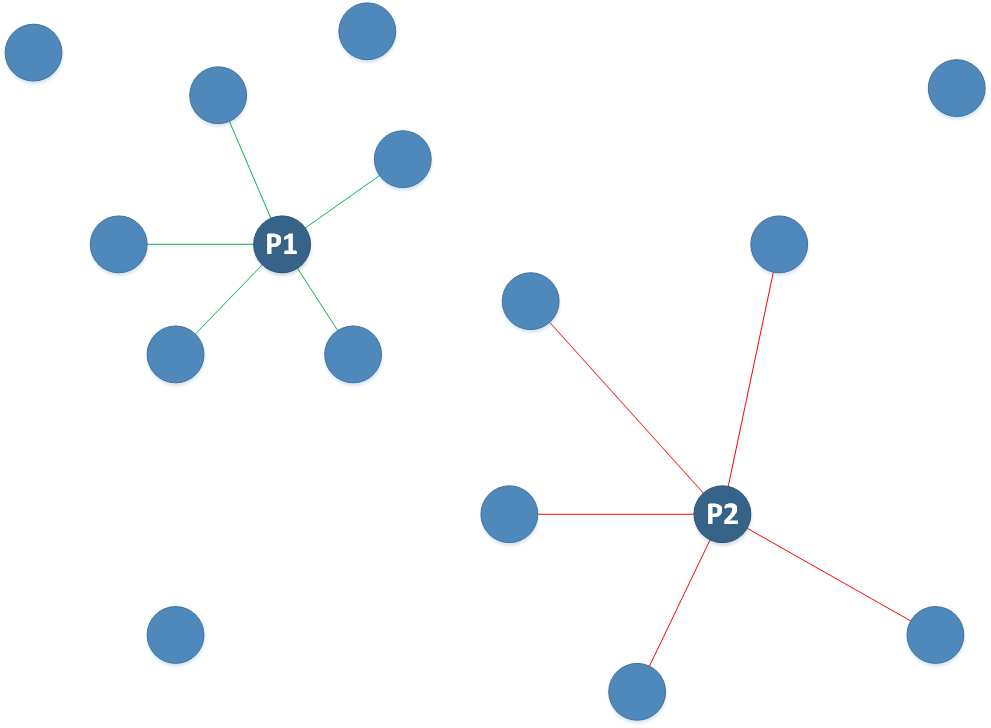
\includegraphics[width=0.8\textwidth]{Imagens/ns_dispersao.png}
		\caption{P1 está em uma região mais densa que P2.}
		\label{fig:ns_dispersao}
	\end{center}
\end{figure}

A geração atual, somada ao arquivo de indivíduos inovadores, fornece uma amostra completa de onde a busca esteve e onde está atualmente; sendo assim, ao tentar maximizar a métrica de inovação, o gradiente de busca se direciona simplesmente ao que é novo, sem qualquer objetivo explícito.

Após substituir a função de avaliação objetiva pela métrica de inovação, o algoritmo evolutivo continua a operar normalmente, selecionando os indivíduos mais inovadores para reprodução. Ao longo das gerações, a população se espalha através do espaço de possíveis comportamentos, algumas vezes encontrando um indivíduo que solucione um dado problema mesmo sem recompensar o progresso em direção à solução do mesmo.

Embora a nota de avaliação não influencie no gradiente de busca na NS, normalmente uma função de avaliação deve ser especificada para identificar os melhores parâmetros de controle para a busca, assim como auxiliar com o critério de parada ao encontrar um indivíduo que satisfaça tal função.

Ao invés de recompensar comportamentos inovadores como na maioria dos experimentos realizados com a NS, semelhante a forma utilizada em \cite{lehman2011evolving}, que analisa o espaço de morfologias de criaturas virtuais, uma nova proposta de explorar o espaço de características fenotípicas, com a finalidade de recompensar características inovadoras que se diferenciam de outras já encontradas, pode melhorar ainda mais os resultados desta metodologia no âmbito desta pesquisa.

\subsection{Minimal Criteria Novelty Search}

A Busca Inovativa com Critério Mínimo (\emph{Minimal Criteria Novelty Search} - MCNS) \cite{lehman2011evolving} é uma extensão da NS que leva em consideração outra característica importante da evolução natural: a função crítica para a evolução de qualquer organismo é a habilidade de sobreviver até ser capaz de se reproduzir.

Para cobrir esta característica, a MCNS implementa um critério mínimo em relação à função de avaliação global, indivíduos que satisfazem tal critério recebem o valor de inovação normalmente, enquanto indivíduos que não satisfazem o critério mínimo recebem o valor zero de inovação e são considerados para a reprodução somente caso nenhum outro indivíduo da população tenha atingido o critério mínimo.

Desta forma o valor de inovação de um indivíduo $i$ na etapa de seleção para reprodução é dada pela equação \ref{eq:ns_inovacao}
\begin{equation}
    \text{inovação}(i) = 
        \begin{cases}
            {disp}_i & \quad \text{se } {nota}_i \geq {cm} \\ 
            0 & \quad \text{caso contrário}\\
       \end{cases}~,
    \label{eq:ns_inovacao}
\end{equation}

\noindent onde ${disp}_i$ é o valor de dispersão calculado para indivíduo de acordo com a equação \ref{eq:ns_dispersao}, ${nota}_i$ sua nota em relação a função de avaliação global e ${cm}$ o critério mínimo predefinido.

Como a nota de avaliação normalmente já é calculada durante a NS, a implementação da MCNS não requer nenhuma tarefa específica nem qualquer medida adicional exceto a filtragem dos indivíduos baseados no valor já obtido.

Após o procedimento de avaliação de critério mínimo a seleção segue normalmente como na NS, selecionando indivíduos com base em suas notas de inovação. A operação de arquivo de indivíduos previamente inovadores não é alterada e funciona da mesma forma que na NS. Mesmo indivíduos que não atingem o critério mínimo são adicionados ao arquivo caso seus valores de inovação sejam bons o suficiente. Isso garante que a busca continue em direção à novos comportamentos sem ficar presos em áreas onde indivíduos não atingem o critério mínimo. A Figura \ref{fig:mcns_diag} apresenta o diagrama de atividades da MCNS.

\begin{figure}[htb]
	\begin{center}
		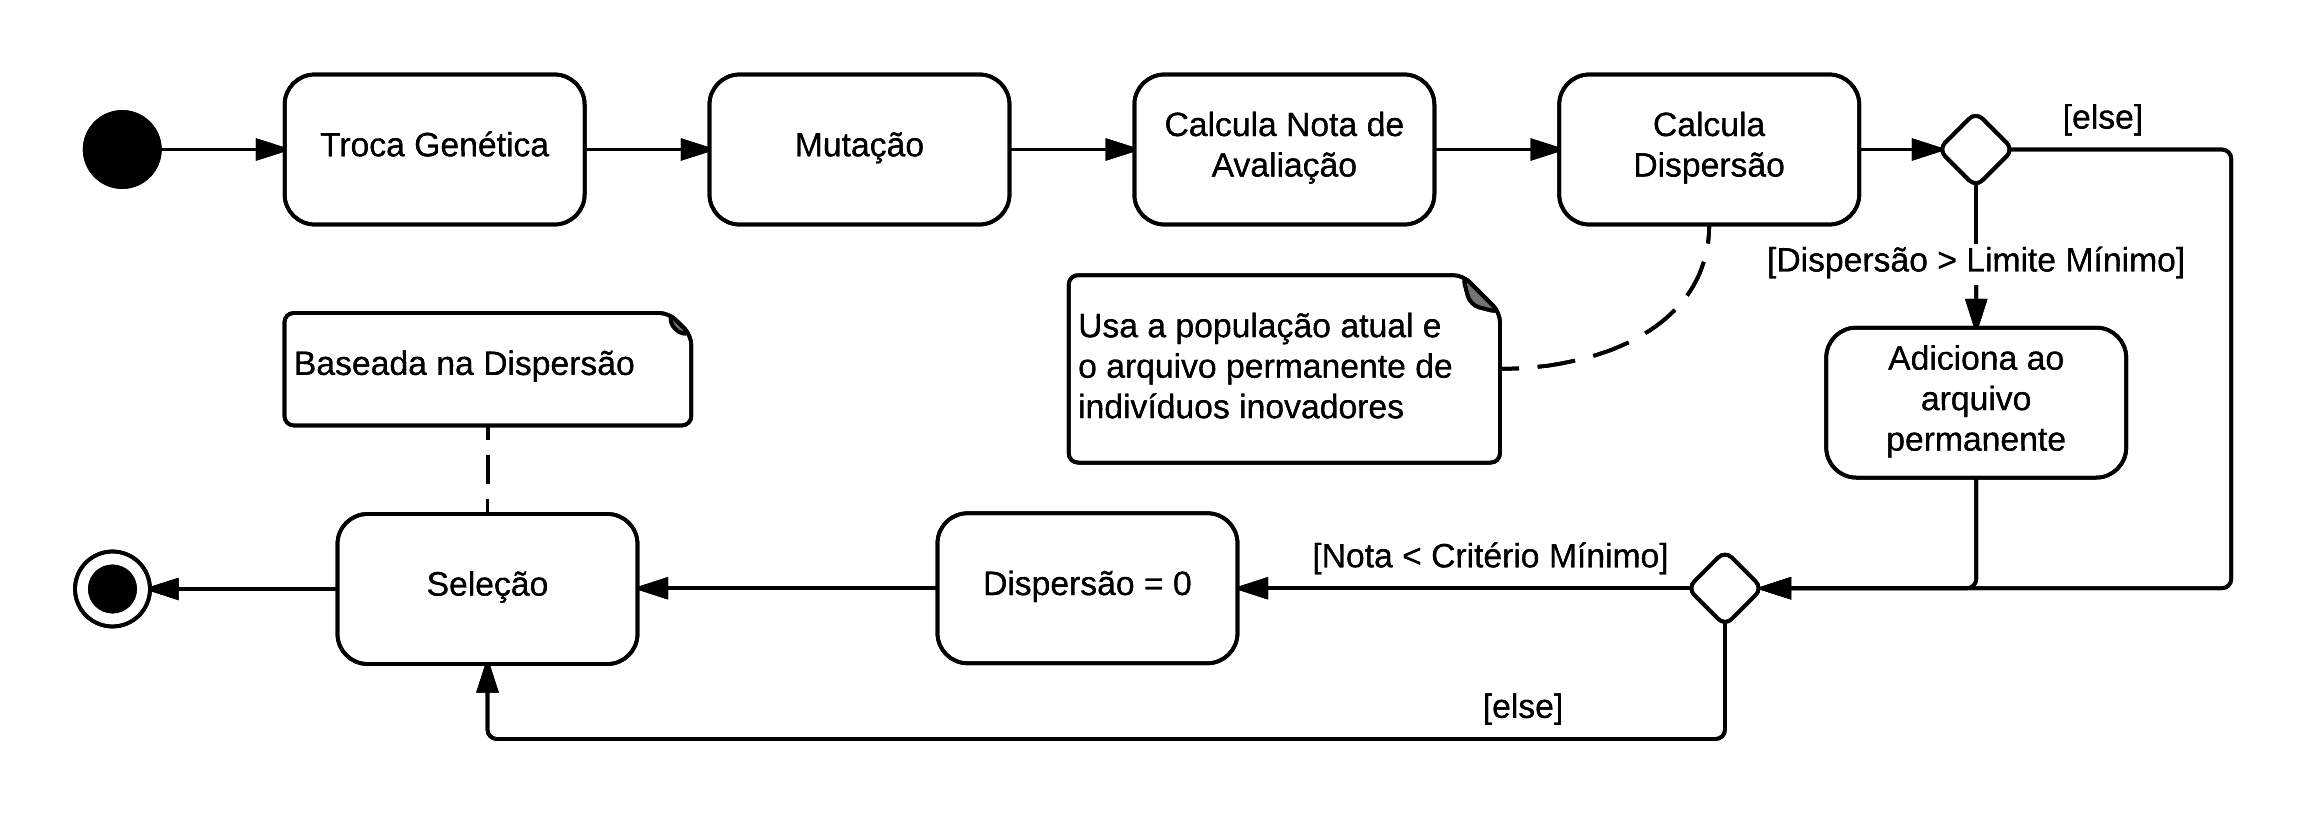
\includegraphics[width=1.0\textwidth]{Imagens/mcns_diag.png}
		\caption{Diagrama de Atividades do Algoritmo Genético de Busca Inovativa com Critério Mínimo.}
		\label{fig:mcns_diag}
	\end{center}
\end{figure}

Como na MCNS os indivíduos que não atingem o critério mínimo são considerados falhas, até que um indivíduo que satisfaça o critério seja encontrado a busca é efetivamente aleatória. Desta forma, se um indivíduo que cumpra o critério não for facilmente encontrado na população inicial pode ser necessário fornecer um genoma previamente evoluído que satisfaça este critério.

\subsection{Progressive Minimal Criteria Novelty Search}

A Busca Inovativa com Critério Mínimo Progresso (\emph{Progressive Minimal Criteria Novelty Search} - PMCNS) \cite{gomes2012progressive} é uma extensão da MCNS que visa aproveitar as restrições do espaço de busca comportamental gerado pela mesma, mas sem a necessidade de predefinir um critério mínimo dependente de domínio. Na PMCNS o limite para o critério mínimo é definido dinamicamente, e assim como na MCNS, somente indivíduos que possuam uma nota de avaliação maior que este limite são considerados para reprodução com seus valores originais de inovação, enquanto indivíduos que não atingirem o critério recebem o valor zero de inovação. Assim como na MCNS, a operação de arquivo de indivíduos previamente inovadores não é alterada.

O critério mínimo é iniciado com um valor mínimo teórico (${cm}_0$) relacionado a função de avaliação (tipicamente zero), desta forma todos os indivíduos iniciais atingem o critério. Em cada nova geração o novo critério mínimo é obtido, inicialmente ordenando-se os indivíduos de forma crescente em relação a suas notas de avaliação e em seguida calculando a posição $n$ através da equação \ref{eq:ns_posicao_n}
\begin{equation}
    n = \frac{P}{100} \times N + \frac{1}{2}~,
    \label{eq:ns_posicao_n}
\end{equation}

\noindent arredondado para o inteiro mais próximo, onde $P$ ($0 \leq P \leq 100$) é a porcentagem predefinida  de indivíduos que devem ficar abaixo do critério mínimo, e $N$ o tamanho da população. O valor $v_n$ é então obtido tomando-se a nota de avaliação da posição $n$ dos valores ordenados.

A fim de restringir progressivamente o espaço de busca, evitando consumir muito tempo com comportamentos com baixas notas de avaliação, o critério mínimo é estritamente crescente e suavemente incrementado com base no valor utilizado na geração anterior de acordo com a equação \ref{eq:ns_cma}
\begin{equation}
    {cm}_g = {cm}_{g-1} + {max}(0,(v_n-{cm}_{g-1}) \times S),
    \label{eq:ns_cma}
\end{equation}

\noindent onde ${cm}$ é o critério mínimo e $S$ ($0 \leq S \leq 1$) o parâmetro de suavização.

O valor de inovação de um indivíduo $i$ na etapa de seleção para reprodução é dada pela equação \ref{eq:pmcns_inovacao}
\begin{equation}
    \text{inovação}(i) = 
        \begin{cases}
            {disp}_i & \quad \text{se } {nota}_i \geq {cm}_g \\ 
            0 & \quad \text{caso contrário}\\
       \end{cases}~,
    \label{eq:pmcns_inovacao}
\end{equation}

\noindent onde ${disp}_i$ é o valor de dispersão calculado para indivíduo de acordo com a equação \ref{eq:ns_dispersao}, ${nota}_i$ sua nota em relação a função de avaliação global e ${cm}_g$ o critério mínimo calculado para a geração atual.

O parâmetro $P$ controla a exigência do critério mínimo: 0 permite que todos indivíduos satisfaçam o critério (assemelhando-se à NS), enquanto 100 restringe o critério mínimo somente ao indivíduo com maior nota. O parâmetro $S$, por sua vez, controla a velocidade de adaptação do critério mínimo: com 0 o critério mínimo não sofre alterações ao longo das gerações, enquanto que com 1 o valor calculado na geração anterior é completamente ignorado.

Com a utilização desta técnica é possível obter os mesmos resultados da NS ou MCNS controlando o parâmetro  $S$ e o valor mínimo teórico inicial ${cm}_0$. Com $S=0$ e ${cm}_0=0$ temos os mesmos resultados da NS, onde todos indivíduos serão sempre aceitos. Alterando ${cm}_0$ e mantendo  $S=0$, obtém-se os mesmos resultados da MCNS, onde ${cm}_0$ não sofrerá alterações ao longo do processo evolutivo e continuará a restringir os indivíduos da mesma forma. Assim sendo, o uso do PMCNS é interessante devido à sua facilidade para comparação entre combinações e técnicas diferentes, além da ausência da necessidade de definição de um parâmetro pré estabelecido dependente de domínio.

\section{NSGA-II}

Algoritmos Evolutivos Multiobjetivo (\emph{Multiobjetive Evolutionary Algorithms} - MOEAs) são uma classe de algoritmos evolutivos que visam resolver problemas de otimização que possuem mais de uma função de avaliação. A presença de vários objetivos em um problema gera um conjunto de soluções ótimas ao invés de uma solução única, este conjunto de soluções é amplamente conhecido como soluções Pareto ótimas. Um bom MOEA deve encontrar o maior número de soluções que sejam o mais próximas das soluções Pareto ótimas possíveis, ao mesmo tempo que \ preserva a diversidade entre as soluções de uma mesma frente não dominada (nichos de soluções).

Soluções Pareto ótimas são aquelas que não são dominadas por nenhuma outra solução, ou seja, sua nota de avaliação para todos os objetivos é sempre maior ou igual às notas de avaliação de quaisquer outras soluções do conjunto. Desta forma, a não ser que mais informações sobre os objetivos sejam fornecidas, não é possível classificar dentre as soluções Pareto ótimas uma que seja considerada a melhor. Por este motivo a diversificação das soluções encontradas em uma mesma frente não dominada é desejável, representando assim as mais variadas possibilidades dentre as soluções encontradas. A Figura \ref{fig:nsgaii_pareto_fronts} apresenta os indivíduos da frente Pareto ótima e de uma segunda frente não dominada em um problema que possui dois objetivos distintos: A e B.

\begin{figure}[htb]
	\begin{center}
		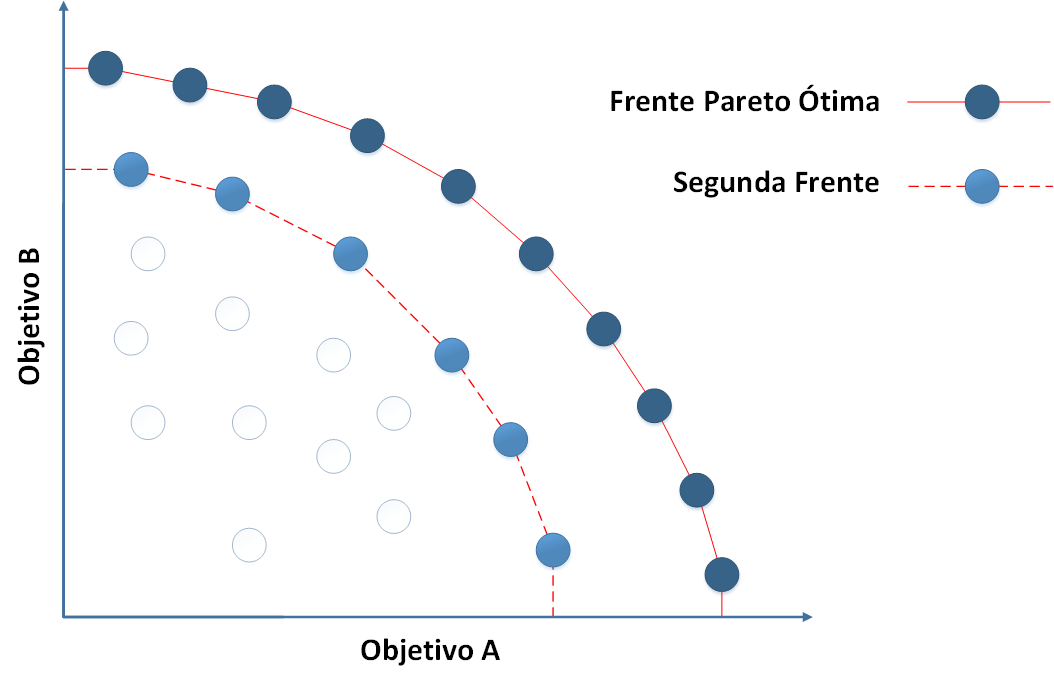
\includegraphics[width=0.8\textwidth]{Imagens/nsgaii_pareto_fronts.png}
		\caption{Frentes não dominadas em um problema multiobjetivo.}
		\label{fig:nsgaii_pareto_fronts}
	\end{center}
\end{figure}

O Algoritmo Genético com Ordenação Não-dominante II (\emph{Nondominated Sorting Genetic Algorithm II} - NSGA-II) é um MOEA proposto em \cite{deb2002fast}, que oferece uma boa distribuição de soluções e uma convergência próxima da fronteira Pareto ótima verdadeira, calculados de forma rápida e eficiente.

O NSGA-II implementa uma ordenação de soluções não dominada, onde cada solução é associada a um conjunto de soluções por ela dominadas e a um contador de soluções que a dominam. As soluções são classificadas de acordo com a frente não dominada em que se encontram. Desta forma, a primeira frente é formada por soluções que não são dominadas por nenhuma outra solução da população; a segunda frente, por sua vez, é constituída por soluções que são dominadas por soluções da primeira frente e que não são dominadas por nenhuma das outras soluções restantes, e assim sucessivamente.

A fim de manter uma boa diversidade e distribuição das soluções dentro das frente não dominadas, o NSGA-II implementa um \emph{operador de comparação de distribuição} (\emph{Crowded-Comparision Operator}) para soluções em frentes não dominadas que não requer parametrização. Essa distribuição é estimada pelo \emph{operador de distância de aglomeração} (\emph{Crowding Distance}), que visa recompensar soluções que estejam em áreas menos densas da frente ao qual pertencem. Soluções dentro de uma mesma frente são classificadas com base na distância média até os pontos vizinhos em ambos os lados e para cada objetivo, calculada pelo perímetro médio do cuboide que envolve uma solução e cujos vértices são os pontos vizinhos na fronteira como mostra a Figura \ref{fig:nsgaii_cuboid}.

\begin{figure}[htb]
	\begin{center}
		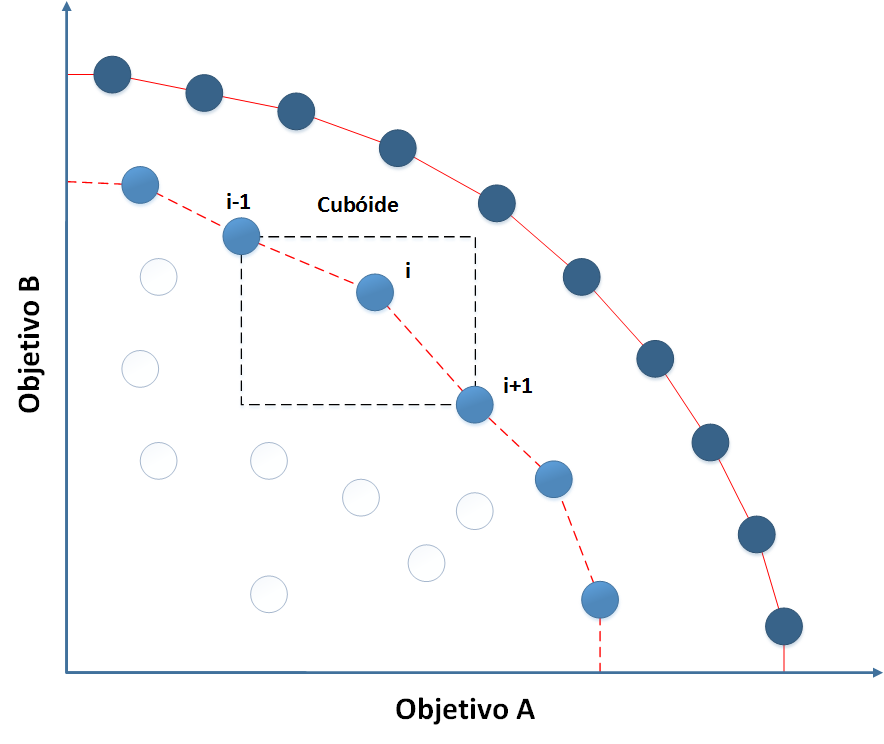
\includegraphics[width=0.8\textwidth]{Imagens/nsgaii_cuboid.png}
		\caption{Representação do cuboide utilizado para o cálculo de distância de aglomeração.}
		\label{fig:nsgaii_cuboid}
	\end{center}
\end{figure}

Assumindo que todo indivíduo $i$ da população possui dois atributos:
\vspace{-5mm}
\begin{enumerate}[leftmargin=1\parindent, noitemsep]
\item Classificação não dominada (${ranque}_i$);
\item Distância de aglomeração (${dist}_i$).
\end{enumerate}
O \emph{operador de comparação de distribuição} ($\prec_n$) é definido pela equação \ref{eq:nsgaii_comparacao_de_distribuicao}
\begin{equation}
    \begin{aligned}
        i\prec_nj & \quad \quad \text{se }({ranque}_i<{ranque}_j) \\
        & \quad \quad \text{ou } (({ranque}_i={ranque}_j) \text{ e }({dist}_i>{dist}_j)).
    \end{aligned}
    \label{eq:nsgaii_comparacao_de_distribuicao}
\end{equation}

Isto é, entre duas soluções com classificação não dominadas diferentes, escolhe-se aquele com menor (melhor) classificação. Caso contrário, se ambas as soluções pertencerem à mesma frente, então escolhe-se a solução localizada em uma região menos aglomerada.

Para gerar uma nova população $P_{t+1}$ de tamanho $N$ a partir de uma geração $t$ qualquer, o NSGA-II combina as populações de progenitores ($P_t$) e descendentes ($Q_t$), os ordena com base no \emph{operador de comparação de distribuição} $\prec_n$ e seleciona os $N$ primeiros indivíduos. Com este procedimento o elitismo é garantido, já que indivíduos da população atual são sempre comparados com indivíduos previamente classificados como sendo as melhores soluções não dominadas até então. A nova população $P_{t+1}$ é então utilizada para seleção, mutação e troca genética na criação da nova população de descendentes $Q_{t+1}$.

A escolha do NSGA-II como MOEA é interessante, pois além de sua velocidade e eficiência, fornece uma função de \emph{distância de aglomeração} (${dist}_i$). Esta, semelhante da forma como foi utilizada por \cite{lehman2011evolving}, pode ser substituída por uma função de distância morfológica, utilizando o valor de dispersão (${disp}_i$) para ordenar uma frente não dominada, sendo capaz de direcionar a diversidade durante a busca para o contexto morfológico em questão.

\section{Diversificação Morfológica}

Algoritmos evolutivos convergem toda a sua população em direção à função de avaliação global, normalmente isso implica em uma população final com indivíduos extremamente semelhantes em algumas de suas características fenotípicas. Esse comportamento ocorre por consequência da natureza do algoritmo evolutivo, que recompensa fortemente nichos onde a nota da função de avaliação é boa. As estratégias a seguir combatem este comportamento de convergência fenotípica e evoluem uma diversidade de criaturas virtuais com somente uma busca.

\subsection{Balanceando Performance e Inovação}

A estratégia utilizada em \cite{lehman2011evolving} emprega as características de exploração por inovação da NS para buscar novos nichos de indivíduos, definindo uma métrica para quantificar a diferença morfológica entre novos indivíduos e indivíduos anteriores.

Com uma métrica de distância puramente morfológica, porém, não é garantido que os indivíduos evoluídos somente com a NS sejam funcionais, ou seja, recompensar somente diferenciação morfológica não visa a melhoria em prol da função de avaliação, garantindo somente a diversidade das características avaliadas em questão e nada mais. Desta forma, uma extensão ao método de NS é proposta, visando contornar a falta de busca objetiva e balanceando duas frentes concorrentes (inovação e performance) com a utilização de um MOEA baseado em eficiência à Pareto. Esta estratégia pode ser vista como uma busca objetiva que encoraja inovação a fim de manter uma diversidade morfológica na população.

Entretanto, a simples combinação de uma função de avaliação global e inovação morfológica em um MOEA não dá suporte ao fato de que: diferentes nichos suportam diferentes níveis de nota de avaliação. Indivíduos em um MOEA baseado em eficiência à Pareto são recompensados com base nas frentes não dominadas. Com isso, em uma frente não dominada com a inovação e a performance como dois objetivos separados, teremos em um extremo indivíduos que maximizam a inovação à custa de performance, enquanto em outro extremo temos indivíduos que maximizam a performance à custa de inovação, e entre ambos os extremos haverão várias combinações e trocas de valores entre performance e inovação. Desta forma, um indivíduo que tenha uma excelente nota de avaliação dentro de seu nicho, mesmo com a nota de avaliação medíocre em relação ao total da população, não será recompensado da forma como deveria.

\subsection{Competição Local}

A solução proposta em \cite{lehman2011evolving} para solucionar o problema de diferentes capacidades dos nichos é: limitar a competição entre indivíduos localmente em relação a seus nichos; ou seja, indivíduos competem entre si somente com outros indivíduos morfologicamente próximos. A ideia é explorar a capacidade dentro de cada nicho ao invés de explorar gananciosamente somente os melhores nichos.

A principal mudança é que a competição local dentro de um nicho transforma a nota de avaliação, que passa de uma medida global para uma medida relativa somente aos vizinhos próximos em seu nicho. Desta forma, o gradiente da busca passa de um balanço entre diversidade e performance global, que beneficia somente alguns nichos, para um balanço entre diversidade e performance dentro de um nicho local.

Na prática, transformar a função de avaliação global em local requer a comparação das performances de um indivíduo em relação a seus vizinhos. Quanto mais vizinhos forem superados maior será sua nota de avaliação local. Assim sendo, a implementação da competição local como uma extensão da NS é simples e direta, uma vez que a NS já calcula os vizinhos mais próximos de cada indivíduo. Durante o cálculo de dispersão, obtido pela média das distâncias entre os vizinhos mais próximos, o número de vizinhos com nota de avaliação menor que o indivíduo em questão é contado. Este número é então atribuído à nota de competição local deste indivíduo, representando sua performance relativa ao seu nicho. A Figura \ref{fig:local_comp_diag} apresenta o diagrama de atividades com as modificações necessárias na NS para a implementação da estratégia de competição local.

\begin{figure}[htb]
	\begin{center}
		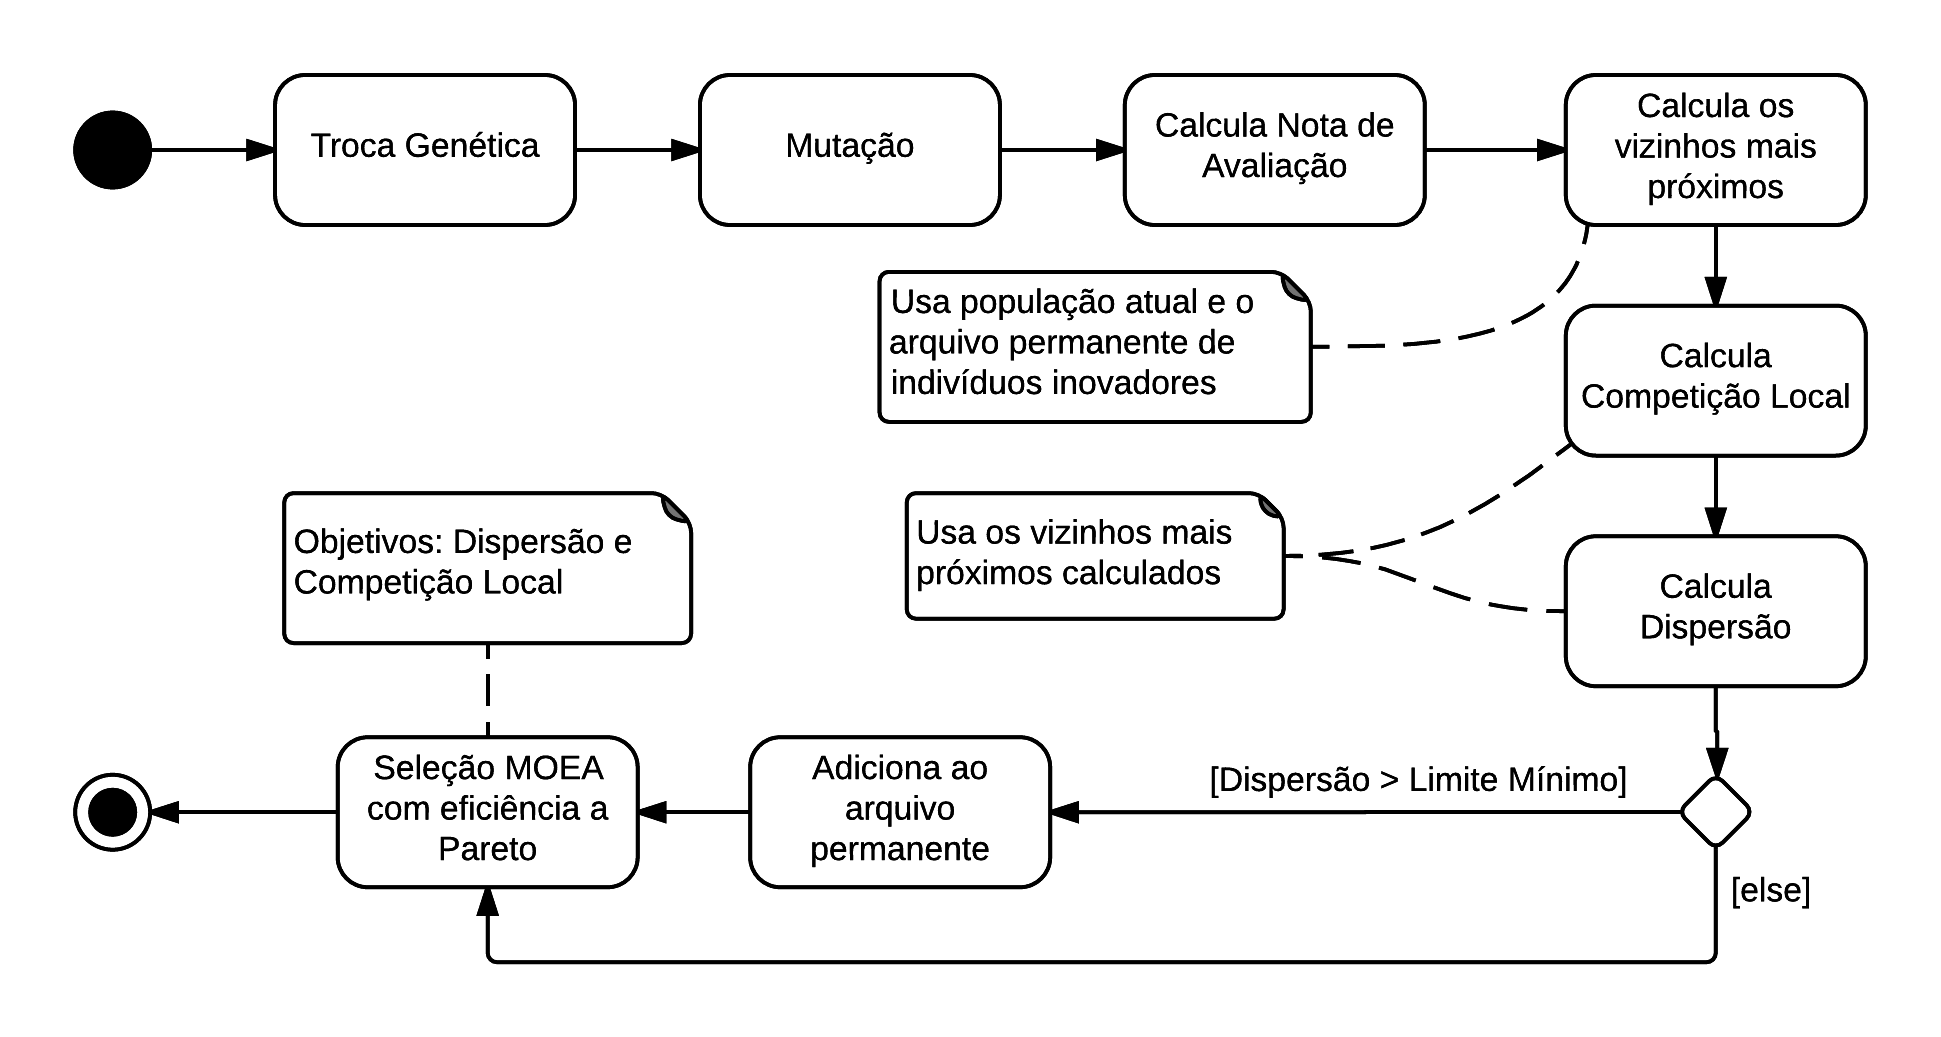
\includegraphics[width=1.0\textwidth]{Imagens/local_comp_diag.png}
		\caption{Diagrama de Atividades para o cálculo de Competição Local em um sistema de Busca Inovativa.}
		\label{fig:local_comp_diag}
	\end{center}
\end{figure}

O valor de competição local é então combinado com o valor de dispersão em um MOEA. Esta nova estratégia pode ser vista como uma busca objetiva limitada a nichos com encorajamento a inovação em busca de novos nichos. Graças às características da eficiência à Pareto, indivíduos com boa nota de avaliação dentro de seus nichos tendem a ser mantidos ao mesmo tempo que indivíduos com altas notas de inovação, motivando assim a exploração e eventualmente encontrando novos nichos a serem otimizados.

Esta estratégia portanto se alinha perfeitamente com os objetivos propostos desta pesquisa: buscar as melhores e mais variadas soluções possíveis para um problema de forma rápida e eficiente. Separando o espaço de busca em nichos garante-se que os indivíduos encontrados serão os mais eficientes dentro de seus respectivos nichos. Com a função de distância é possível controlar quais serão as características diferenciais destes nichos, tipicamente características fenotípicas nas quais desejamos diversificação; no caso de \cite{lehman2011evolving} esta característica fenotípica é a morfologia das criaturas virtuais obtidas, e na aplicação escolhida para esta pesquisa são as características visuais e estruturais dos mapas gerados automaticamente.